\chapter{Lý Thuyết Data Fitting và Minh Họa}

\newpage

\section{Bài Toán Data Fitting và Mô Hình Hồi Quy Tuyến Tính}

\subsection{Bài toán tổng quát}

Trong các nghiên cứu về thực nghiệm và khoa học dữ liệu, ta thường xuyên gặp bài toán xấp xỉ hàm để tìm ra quy luật mô tả mối quan hệ giữa các biến số. Giả sử, ta có một tập dữ liệu gồm $n$ quan sát như sau:

\begin{equation}
    \mathcal{D} = \{(x_{i1}, x_{i2}, \dots, x_{ip}, y_i)\}_{i=1}^n
\end{equation}

Trong đó:

\begin{itemize}[topsep=0pt, itemsep=2.5pt, leftmargin=1.5cm]
    \item $y_i \in \mathbb{R}$ là biến phụ thuộc hay là biến mục tiêu cần dự đoán.
    \item $X_i = (x_{i_1}, x_{i_2}, \dots, x_{i_p}) \in \mathbb{R}^p$ là vector gồm $p$ biến độc lập hay là biến giải thích.
\end{itemize}

Mục tiêu của bài toán là tìm một hàm số toán học $f(X)$ đóng vai trò xấp xỉ tốt nhất các giá trị $y_i$, tức là $y_i \approx f(X_i)$.

\subsection{Mô Hình Hồi Quy Tuyến Tính}

Xét một trong những mô hình phổ biến và nền tảng nhất chính là \textbf{Mô hình hồi quy tuyến tính bội}. Mô hình giả định mối quan hệ giữa các biến phụ thuộc và các biến độc lập là tuyến tính đối với các tham số. Mô hình được biểu diễn dưới dạng các phương trình đại số sau với mỗi quan sát $i$:

\begin{equation}
    y_i = \beta_0 + \beta_1 x_{i_1} + \beta_2 x_{i_2} + \dots + \beta_p x_{i_p} + \epsilon_i, \forall i = 1, 2, \dots, n
\end{equation}

Trong đó:

\begin{itemize}[topsep=0pt, itemsep=2.5pt, leftmargin=1.5cm]
    \item $\beta_0$ là hệ số chặn (Intercept).
    \item $\beta_1, \beta_2, \dots, \beta_p$ là các hệ số hồi quy ứng với từng biến độc lập.
    \item $\epsilon_i$ là sai số ngẫu nhiên (nhiễu - noise) đại diện cho phần biến động của $y_i$ mà các biến độc lập trong mô hình không giải thích được.
\end{itemize}

Hệ phương trình gồm $n$ dòng trên được tổng quát hóa dưới dạng ma trận để thuận tiện cho việc biến đổi toán học và tính toán:

\begin{equation}
    \mathbf{y} = X\beta + \epsilon
\end{equation}

Định nghĩa chi tiết các thành phần trong phương trình trên:

\begin{itemize}[topsep=0pt, itemsep=2.5pt, leftmargin=1.5cm]
    \item $y \in \mathbb{R}^{n \times 1}$ là vector cột chứa các giá trị của biến phụ thuộc.

    $$\mathbf{y} = \begin{bmatrix} y_1 \\ y_2 \\ \vdots \\ y_n \end{bmatrix}$$

    \item $X \in \mathbb{R}^{n \times (p + 1)}$ là ma trận thiết kế (Design Matrix) với cột đầu tiên chứa toàn hệ số 1 nhằm tích hợp hệ số chặn $\beta_0$ vào phép nhân ma trận.

    $$\mathbf{X} = \begin{bmatrix} 1 & x_{11} & x_{12} & \dots & x_{1p} \\ 1 & x_{21} & x_{22} & \dots & x_{2p} \\ \vdots & \vdots & \vdots & \ddots & \vdots \\ 1 & x_{n1} & x_{n2} & \dots & x_{np} \end{bmatrix}$$

    \item $\beta \in \mathbb{R}^{(p + 1) \times 1}$ là vector cột chứa toàn bộ hệ số cần ước lượng.

    $$\boldsymbol{\beta} = \begin{bmatrix} \beta_0 \\ \beta_1 \\ \vdots \\ \beta_p \end{bmatrix}$$

    \item $\epsilon \in \mathbb{R}^{n \times 1}$ là vector cột chứa các sai số ngẫu nhiên.

    $$\boldsymbol{\varepsilon} = \begin{bmatrix} \varepsilon_1 \\ \varepsilon_2 \\ \vdots \\ \varepsilon_n \end{bmatrix}$$
\end{itemize}

\section{Phương Pháp Bình Phương Tối Tiểu}

\subsection{Hàm mất mát (Loss Function)}

Ý tưởng cốt lõi của phương pháp bình phương tối tiểu (Ordinary Least Squares - OLS) là tìm kiếm vector tham số ước lượng $\hat{\beta}$ sao cho tổng bình phương các khoảng cách sai lệch giữa các giá trị thực tế $y_i$ và giá trị dự báo $\hat{y}_i$ đạt giá trị nhỏ nhất. Tổng bình phương các khoảng cách trên được gọi là \textbf{Tổng bình phương phần dư} (Residual Sum Of Squares - RSS):

\begin{equation}
    RSS(\boldsymbol{\beta}) = \sum_{i=1}^{n} (y_i - \hat{y}_i)^2 = \sum_{i=1}^{n} (y_i - \mathbf{x}_i^T\boldsymbol{\beta})^2
\end{equation}

Biểu diễn dưới ma trận và chuẩn $L_2$, hàm mất mát có dạng:

\begin{equation}
    RSS(\boldsymbol{\beta}) = \|\mathbf{y} - \mathbf{X}\boldsymbol{\beta}\|_2^2 = (\mathbf{y} - \mathbf{X}\boldsymbol{\beta})^T(\mathbf{y} - \mathbf{X}\boldsymbol{\beta})
\end{equation}

\subsection{Chứng minh nghiệm cực tiểu}

Để tìm cực tiểu của hàm mất mát trên, ta tiến hành triển khai đại số biểu thức ma trận trên:

\vspace{-0.5em}

\begin{align}
    RSS(\boldsymbol{\beta}) &= (\mathbf{y}^T - \boldsymbol{\beta}^T\mathbf{X}^T)(\mathbf{y} - \mathbf{X}\boldsymbol{\beta}) \\
    RSS(\boldsymbol{\beta}) &= \mathbf{y}^T\mathbf{y} - \mathbf{y}^T\mathbf{X}\boldsymbol{\beta} - \boldsymbol{\beta}^T\mathbf{X}^T\mathbf{y} + \boldsymbol{\beta}^T\mathbf{X}^T\mathbf{X}\boldsymbol{\beta}
\end{align}

Vì $\mathbf{y}^T\mathbf{X}\boldsymbol{\beta}$ là một đại lượng vô hướng (scalar), nó bằng với chuyển vị của chính nó: $(\mathbf{y}^T\mathbf{X}\boldsymbol{\beta})^T = \boldsymbol{\beta}^T\mathbf{X}^T\mathbf{y}$. Do đó, ta thu gọn được hàm mất mát thành:

\begin{equation}
    RSS(\boldsymbol{\beta}) = \mathbf{y}^T\mathbf{y} - 2\boldsymbol{\beta}^T\mathbf{X}^T\mathbf{y} + \boldsymbol{\beta}^T\mathbf{X}^T\mathbf{X}\boldsymbol{\beta}
\end{equation}

Tiến hành lấy đạo hàm ma trận (Matrix Calculus) của hàm số theo vector tham số $\boldsymbol{\beta}$:

\begin{equation}
    \frac{\partial RSS(\boldsymbol{\beta})}{\partial \boldsymbol{\beta}} = \mathbf{0} - 2\mathbf{X}^T\mathbf{y} + 2\mathbf{X}^T\mathbf{X}\boldsymbol{\beta}
\end{equation}

Để tìm điểm cực trị, ta thiết lập đạo hàm này bằng vector không $\mathbf{0}$:

\begin{equation}
    -2\mathbf{X}^T\mathbf{y} + 2\mathbf{X}^T\mathbf{X}\boldsymbol{\beta} = \mathbf{0} \implies \mathbf{X}^T\mathbf{X}\boldsymbol{\beta} = \mathbf{X}^T\mathbf{y}
\end{equation}

Phương trình trên được gọi là hệ Phương trình chuẩn tắc (Normal Equations) trong lý thuyết bình phương tối tiểu.

Để phương trình trên có nghiệm thì ma trận $X^T X$ phải khả nghịch. Khi đó, ta thu được công thức nghiệm duy nhất cho ước lượng OLS:

\begin{equation}
    \hat{\boldsymbol{\beta}}_{OLS} = (\mathbf{X}^T\mathbf{X})^{-1}\mathbf{X}^T\mathbf{y}
\end{equation}

\section{Các Giả Thiết Gauss-Markov và Định lý Gauss-Markov}

\subsection{Các Giả Thiết Gauss-Markov}

Để phương pháp ước lượng bình phương tối tiểu (OLS) đạt được những tính chất thống kê tối ưu và các suy diễn kiểm định có hiệu lực thì mô hình phải bắt buộc thỏa mãn cả 5 giả thuyết Gauss-Markov sau đây:

\begin{enumerate}[topsep=0pt, itemsep=2.5pt, leftmargin=1.5cm]
    \item Tuyến tính trong tham số (Linear in Parameters): Mối quan hệ giữa $\mathbf{y}$ và $\mathbf{X}$ được biểu diễn đúng dưới dạng tuyến tính $\mathbf{y} = \mathbf{X}\boldsymbol{\beta} + \boldsymbol{\varepsilon}$.

    \item Không có đa cộng tuyến hoàn hảo (No Perfect Collinearity): Ma trận thiết kế $\mathbf{X}$ có hạng đầy đủ cột, nghĩa là $\text{rank}(\mathbf{X}) = p+1 < n$. Giả thiết này đảm bảo các cột của $\mathbf{X}$ độc lập tuyến tính với nhau, dẫn đến ma trận vuông $\mathbf{X}^T\mathbf{X}$ là một ma trận khả nghịch (không bị suy biến).

    \item Kỳ vọng nhiễu bằng 0 (Zero Conditional Mean): Kỳ vọng của vector sai số khi biết ma trận thiết kế bằng vector không:

    $$E[\boldsymbol{\varepsilon} | \mathbf{X}] = \mathbf{0}$$

    Giả thiết này khẳng định sai số không chứa thông tin hệ thống và không có mối tương quan với các biến độc lập.

    \item Phương sai nhiễu thuần nhất (Homoscedasticity): Phương sai của sai số ngẫu nhiên tại mọi quan sát là hằng số không đổi:

    $$\text{Var}(\varepsilon_i | \mathbf{X}) = \sigma^2, \quad \forall i = 1, 2, \dots, n$$

    \item Không có tự tương quan giữa các sai số (No Autocorrelation): Hiệp phương sai giữa hai sai số của hai quan sát khác nhau bất kỳ luôn bằng 0:
    
    $$\text{Cov}(\varepsilon_i, \varepsilon_j | \mathbf{X}) = 0, \quad \forall i \neq j$$
\end{enumerate}

Từ hai giả thuyết (4) và (5), ma trận hiệp phương sai của vector phần dư $\epsilon$ có dạng đơn vị hóa:

$$\text{Var}(\boldsymbol{\varepsilon} | \mathbf{X}) = \sigma^2 \mathbf{I}_n$$

Trong đó, $\mathbf{I}_n$ là ma trận đơn vị kích thước $n \times n$.

\subsection{Định lý Gauss-Markov}

\begin{theorem}
    Nếu một mô hình hồi quy tuyến tính thỏa mãn đầy đủ các giả thiết từ (1) đến (5), thì ước lượng Bình phương Nhỏ nhất $\hat{\boldsymbol{\beta}}_{OLS}$ là ước lượng tuyến tính không chệch tốt nhất — BLUE (Best Linear Unbiased Estimator).
\end{theorem}

"Tốt nhất" mang ý nghĩa là trong tất cả các ước lượng tuyến tính và không chệch của $\beta$, ước lượng OLS là ước lượng đạt phương sai nhỏ nhất ($\text{Var}(\hat{\boldsymbol{\beta}}_{OLS}) \le \text{Var}(\tilde{\boldsymbol{\beta}})$ với mọi ước lượng không chệch $\tilde{\boldsymbol{\beta}}$ khác) nằm đảm bảo tính ổn định và tin cậy vượt trội của nghiệm OLS khi áp dụng trên thực nghiệm.

\section{Ma Trận Chiếu (Hat Matrix) và Tính Chất Hình Học của OLS}

\subsection{Định nghĩa}

Sau khi thu được nghiệm tối ưu $\hat{\boldsymbol{\beta}}_{OLS}$, vector các giá trị dự báo $\hat{\mathbf{y}}$ được tính toán qua công thức:

\begin{equation}
    \hat{\mathbf{y}} = \mathbf{X}\hat{\boldsymbol{\beta}}_{OLS} = \mathbf{X}(\mathbf{X}^T\mathbf{X})^{-1}\mathbf{X}^T\mathbf{y}
\end{equation}

Đặt ma trận, $\mathbf{H} = \mathbf{X}(\mathbf{X}^T\mathbf{X})^{-1}\mathbf{X}^T$, khi đó các giá trị dự báo có thể được viết lại dưới dạng:

\begin{equation}
    \hat{\mathbf{y}} = \mathbf{H}\mathbf{y}
\end{equation}

Ma trận $H$ được gọi là \textbf{Ma trận mũ} (Hat Matrix) với vai trò biến vector quan sát thực tế $\mathbf{y}$ thành vector ước lượng $\hat{\mathbf{y}}$.

\subsection{Tính chất}

\subsubsection{Tính đối xứng (Symmetry)}

\begin{equation}
    H^T = H
\end{equation}

\noindent Chứng minh: $$\mathbf{H}^T = \left[ \mathbf{X}(\mathbf{X}^T\mathbf{X})^{-1}\mathbf{X}^T \right]^T = (\mathbf{X}^T)^T \left[ (\mathbf{X}^T\mathbf{X})^{-1} \right]^T \mathbf{X}^T$$

Vì $(\mathbf{X}^T)^T = \mathbf{X}$ và ma trận tích $\mathbf{X}^T\mathbf{X}$ là một ma trận đối xứng ($\left(\mathbf{X}^T\mathbf{X}\right)^T = \mathbf{X}^T\mathbf{X}$), nên ma trận nghịch đảo của nó cũng là ma trận đối xứng, tức là $\left[ (\mathbf{X}^T\mathbf{X})^{-1} \right]^T = (\mathbf{X}^T\mathbf{X})^{-1}$. Do đó, ta thu được:

\begin{equation}
    \mathbf{H}^T = \mathbf{X}(\mathbf{X}^T\mathbf{X})^{-1}\mathbf{X}^T = \mathbf{H} \quad (\text{đpcm})
\end{equation}

\subsubsection{Tính lũy đẳng (Idempotency)}

\begin{equation}
    H^2 = H
\end{equation}

\noindent Chứng minh: Nhân ma trận $\mathbf{H}$ với chính nó

\begin{align}
    \mathbf{H}^2 = \mathbf{H}\mathbf{H} &= \left[ \mathbf{X}(\mathbf{X}^T\mathbf{X})^{-1}\mathbf{X}^T \right] \left[ \mathbf{X}(\mathbf{X}^T\mathbf{X})^{-1}\mathbf{X}^T \right] \\ 
    \mathbf{H}^2 &= \mathbf{X} \cdot \underbrace{\left[(\mathbf{X}^T\mathbf{X})^{-1} (\mathbf{X}^T\mathbf{X})\right]}_{\mathbf{I}_{p+1}} \cdot (\mathbf{X}^T\mathbf{X})^{-1}\mathbf{X}^T
\end{align}

Vì $\mathbf{I}_{p+1}$ là ma trận đơn vị kích thước $(p+1) \times (p+1)$, ta có:

$$\mathbf{H}^2 = \mathbf{X} \cdot \mathbf{I}_{p+1} \cdot (\mathbf{X}^T\mathbf{X})^{-1}\mathbf{X}^T = \mathbf{X}(\mathbf{X}^T\mathbf{X})^{-1}\mathbf{X}^T = \mathbf{H} \quad (\text{đpcm})$$

\subsubsection{Vết của ma trận (Trace property)}

\begin{equation}
    \text{trace}(\mathbf{H}) = p + 1
\end{equation}

\noindent Chứng minh:

\vspace{-0.5em}

\begin{align}
    \text{trace}(\mathbf{H}) &= \text{trace}\left( \mathbf{X} \cdot \left[(\mathbf{X}^T\mathbf{X})^{-1}\mathbf{X}^T\right] \right) = \text{trace}\left( \left[(\mathbf{X}^T\mathbf{X})^{-1}\mathbf{X}^T\right] \cdot \mathbf{X} \right) \\ 
    \text{trace}(\mathbf{H}) &= \text{trace}\left( (\mathbf{X}^T\mathbf{X})^{-1} (\mathbf{X}^T\mathbf{X}) \right) = \text{trace}(\mathbf{I}_{p+1}) = p + 1 \quad (\text{đpcm})
\end{align}

\subsection{Ý nghĩa hình học}

\subsubsection{Không gian con tuyến tính của các biến độc lập}

Xét ma trận thiết kế $\mathbf{X} \in \mathbb{R}^{n \times (p+1)}$ gồm vector biến độc lập $X_1, X_2, \dots, X_p$. Tập hợp tất cả các tổ hợp tuyến tính của các cột trên sẽ tạo thành một không gian con (Subspace), được gọi là \textbf{Không gian cột} của $\mathbf{X}$, ký hiệu là $\text{Col}(\mathbf{X}) \subset \mathbb{R}^n$. Chiều của không gian con bằng $\text{rank}(\mathbf{X}) = p+1$.

Vector dữ liệu thực tế quan sát $\mathbf{y} \in \mathbb{R}^n$ là một điểm trong không gian $n$ chiều. Tuy nhiên, do sự tác động ngẫu nhiên của nhiễu $\epsilon$ nên vector $\mathbf{y}$ hầu như luôn nằm ngoài không gian con $\text{Col}(\mathbf{X})$.

\subsubsection{Mục tiêu hình học và Vector phần dư}

Bất kỳ vector dự báo $\hat{\mathbf{y}}$ do mô hình tạo ra đều bắt buộc phải nằm trong không gian con $\text{Col}(\mathbf{X})$ do $\hat{\mathbf{y}} = \mathbf{X}\hat{\boldsymbol{\beta}}$.

Do đó, bài toán tối thiểu tổng bình phương phần dư $RSS = \|\mathbf{y} - \hat{\mathbf{y}}\|_2^2$ tương đương với bài toán hình học: Tìm một điểm $\hat{\mathbf{y}}$ thuộc không gian con $\text{Col}(\mathbf{X})$ sao cho khoảng cách Euclide từ điểm $\mathbf{y}$ đến nó là ngắn nhất.

Khoảng cách từ một điểm đến một mặt phẳng (không gian con) đạt giá trị nhỏ nhất khi và chỉ khi đoạn thẳng nối giữa chúng vuông góc với mặt phẳng đó. Khi đó, vector $\mathbf{e} = \mathbf{y} - \hat{\mathbf{y}}$ phải vuông góc hoàn toàn với mọi vector nằm trong $\text{Col}(\mathbf{X})$.

Điều kiện vuông góc được biểu diễn dưới dạng tích vô hướng như sau:

\begin{equation}
    \mathbf{X}^T\mathbf{e} = \mathbf{0} \implies \mathbf{X}^T(\mathbf{y} - \hat{\mathbf{y}}) = \mathbf{0} \implies \mathbf{X}^T\mathbf{y} = \mathbf{X}^T\mathbf{X}\hat{\boldsymbol{\beta}}
\end{equation}

Đây chính là cách giải thích hình học trực quan tại sao ta thu được kết quả nghiệm đóng của ước lượng OLS.

\subsubsection{Vai trò toán tử chiếu của Hat Matrix}

Ma trận $\mathbf{H}$ chính là toán tử chiếu vuông góc. Khi ta thực hiện phép nhân ma trận $\hat{\mathbf{y}} = \mathbf{H}\mathbf{y}$, ma trận $\mathbf{H}$ sẽ chiếu vuông góc từ đầu mút của vector $\mathbf{y}$ xuống không gian con $\text{Col}(\mathbf{X})$ để tìm ra vị trí tọa độ tối ưu $\hat{\mathbf{y}}$.

Mối liên hệ giữa tính chất của ma trận chiếu với ý nghĩa hình học:

\begin{itemize}[topsep=0pt, itemsep=2.5pt, leftmargin=1.5cm]
    \item Tính đối xứng: Đảm bảo cho phép chiếu vuông góc không trở thành phép chiếu xiên, làm khoảng cách từ $\mathbf{y}$ đến không gian con là ngắn nhất.
    \item Tính lũy đẳng: Khi vector $\mathbf{y}$ đã được chiếu vuông góc xuống không gian con $\text{Col}(\mathbf{X})$ để trở thành $\hat{\mathbf{y}}$, điểm $\hat{\mathbf{y}}$ này đã nằm sẵn trên mặt phẳng. Nếu ta tiếp tục dùng toán tử $\mathbf{H}$ để chiếu nó lần thứ hai, vị trí của nó sẽ đứng yên không thay đổi ($\mathbf{H}\hat{\mathbf{y}} = \hat{\mathbf{y}}$).
    \item Tính chất vết ($\text{trace}(\mathbf{H}) = p + 1$): Vết của một ma trận chiếu vuông góc trong đại số tuyến tính luôn luôn bằng số chiều (dimension) của không gian con mà nó chiếu xuống. Trong bài toán hồi quy bội, số chiều này chính là số lượng tham số độc lập cần ước lượng ($p+1$).
\end{itemize}

\section{Các Chỉ Số Đánh Giá Mô Hình}

Để định lượng hiệu năng và đo lường độ chính xác của hàm xấp xỉ dữ liệu thu được, lý thuyết hồi quy xây dựng một hệ thống các chỉ số đánh giá dựa trên việc phân rã tổng bình phương biến động (Sum of Squares Decomposition).


\begin{table}[H]
    \centering
    \renewcommand{\arraystretch}{1.5}
    \setlength{\tabcolsep}{8pt}
    
    \begin{tabular}{|p{3.5cm}|p{5.5cm}|p{6cm}|}
        \hline
        \rowcolor[rgb]{0.8, 0.9, 1.0}
        \textbf{Chỉ số} & \textbf{Công thức toán học} & \textbf{Ý nghĩa} \\ \hline
        
        \textbf{TSS} (Total Sum of Squares) & $TSS = \sum_{i=1}^n (y_i - \bar{y})^2$ & Đo lường toàn bộ sự biến động của biến phụ thuộc $y$ xung quanh giá trị trung bình mẫu $\bar{y}$ khi chưa có mô hình hồi quy. \\ \hline
        
        \textbf{ESS} (Explained Sum of Squares) & $ESS = \sum_{i=1}^n (\hat{y}_i - \bar{y})^2$ & Phần biến động của biến mục tiêu được giải thích thành công bởi quy luật tuyến tính của các biến độc lập trong mô hình. \\ \hline
        
        \textbf{RSS} (Residual Sum of Squares) & $RSS = \sum_{i=1}^n (y_i - \hat{y}_i)^2$ & Phần sai lệch biến động còn sót lại do nhiễu ngẫu nhiên hoặc do mô hình bỏ sót biến, không thể giải thích được. \\ \hline

        \textbf{MAE} (Mean Absolute Error) & $MAE = \frac{1}{n} \sum_{i=1}^n \|y_i - \hat{y}_i\|$ & Giá trị trung bình của các sai lệch tuyệt đối giữa giá trị thực tế và giá trị dự báo. \\ \hline

        \textbf{RMSE} (Root Mean Squared Error) & $RMSE = \sqrt{\frac{1}{n} \sum_{i=1}^n (y_i - \hat{y}_i)^2}$ & Căn bậc hai của trung bình bình phương các sai lệch (độ lệch chuẩn của phần dư). \\ \hline
    \end{tabular}
    \caption{Các chỉ số đo lường sự biến động trong mô hình hồi quy}
\end{table}


Mối quan hệ toán học nền tảng giữa ba chỉ số: $TSS = ESS + RSS$.

\begin{itemize}[topsep=0pt, itemsep=2.5pt, leftmargin=1.5cm]
    \item Hệ số xác định $R^2$:

    $$R^2 = \frac{ESS}{TSS} = 1 - \frac{RSS}{TSS}$$

    Chỉ số $R^2 \in [0, 1]$ biểu thị tỷ lệ phần trăm sự biến động của dữ liệu thực tế được giải thích bởi mô hình. $R^2$ càng tiến gần tới 1 chứng tỏ hàm xấp xỉ càng khớp với dữ liệu thực nghiệm.

    \item Hệ số xác định hiệu chỉnh $\bar{R}^2$

    Vì giá trị của $R^2$ luôn có xu hướng tăng lên hoặc giữ nguyên nếu xuất hiện thêm biến độc lập mới vào $\mathbf{X}$ dù cho biến mới đó không có ý nghĩa nên để giải quyết vấn đề overfitting thì $\bar{R}^2$ thêm cơ chế phạt dựa trên số lượng tham số $p$ hiện có:

    $$\bar{R}^2 = 1 - \left[ \frac{RSS/(n - p - 1)}{TSS/(n - 1)} \right]$$

    \item Thống kê kiểm định F: Được sử dụng nhằm đánh giá ý nghĩa thống kê của toàn bộ mô hình tổng thể. Chỉ số này kiểm tra cặp giả thuyết:

    \begin{itemize}[label=\ding{111}, leftmargin=1.5cm]
        \item $H_0: \beta_1 = \beta_2 = \dots = \beta_p = 0$ (Tất cả các biến độc lập đều không có tác động).
        \item $H_1$: Tồn tại ít nhất một hệ số $\beta_j \neq 0$ (Mô hình có ý nghĩa ít nhất với 1 biến).
    \end{itemize}

    Công thức toán học giá trị thống kê $F$:

    $$F = \frac{ESS / p}{RSS / (n - p - 1)}$$

\end{itemize}

\section{Suy Diễn Thống Kê Cho Các Hệ Số}

Để mở rộng bài toán hồi quy từ mức độ mô tả sang mức độ suy diễn thống kê tức là xác định xem một biến độc lập có thực sự ảnh hưởng đến biến phụ thuộc hay không, ta tiến hành kiểm định thống kê cho từng hệ số $\beta_j$.

Dưới giả thiết chuẩn GM5, ta có phân phối chuẩn của sai số:

\begin{equation}
    \boldsymbol{\varepsilon} | \mathbf{X} \sim \mathcal{N}(\mathbf{0}, \sigma^2 \mathbf{I}_n)
\end{equation}

\subsection{Phân phối mẫu của ước lượng OLS}

Vì nghiệm $\hat{\boldsymbol{\beta}}_{OLS}$ là một phép biến đổi tuyến tính của vector $\mathbf{y}$ nên vector ước lượng $\hat{\beta}$ cũng tuân theo phân phối chuẩn:

\begin{equation}
    \hat{\boldsymbol{\beta}}_{OLS} \sim \mathcal{N}\left( \boldsymbol{\beta}, \sigma^2 (\mathbf{X}^T\mathbf{X})^{-1} \right)
\end{equation}

Do phương sai nhiễu $\sigma^2$ trong thực tế không biết trước, ta sử dụng một ước lượng không chệch của nó trích xuất từ phương sai phần dư mẫu:

$$\hat{\sigma}^2 = \frac{RSS}{n - p - 1}$$

Khi đó, ma trận hiệp phương sai mẫu của các hệ số hồi quy được tính bằng:

$$\widehat{\text{Var}}(\hat{\boldsymbol{\beta}}_{OLS}) = \hat{\sigma}^2 (\mathbf{X}^T\mathbf{X})^{-1}$$

\subsection{Kiểm định t-test và khoảng tin cậy}

Sai số chuẩn (Standard Error): Căn bậc hai của các phần tử nằm trên đường chéo chính của ma trận $\widehat{\text{Var}}(\hat{\boldsymbol{\beta}}_{OLS})$ chính là sai số chuẩn của từng hệ số hồi quy đơn lẻ, ký hiệu là $SE(\hat{\beta}_j)$.

Kiểm định giả thuyết t-test: Để đánh giá xem một biến độc lập $x_j$ cụ thể nào đó có thực sự đóng góp ý nghĩa vào việc giải thích biến phụ thuộc $y$ hay không, ta thực hiện kiểm định giả thuyết riêng lẻ:

$$H_0: \beta_j = 0 \quad ; \quad H_1: \beta_j \neq 0$$

Thống kê kiểm định t được xây dựng theo công thức: $$t_j = \frac{\hat{\beta}_j}{SE(\hat{\beta}_j)}$$

Dưới giả thuyết $H_0$, giá trị $t_j$ tuân theo phân phối Student $t$ với bậc tự do là $(n - p - 1)$, từ đó ta tính ra giá trị xác suất \textbf{p-value}. Nếu $\text{p-value} < \alpha$ với mức nghĩa $\alpha = 0.05$ thì ta bác bỏ giả thuyết $H_0$ và kết luận biến đó có ý nghĩa thống kê.

Khoảng tin cậy (Confidence Interval): Khoảng tin cậy cấu thành mức độ dao động khả thi của tham số thực tế ở mức tin cậy $(1 - \alpha)$ được xác định bởi phương trình:

$$\left[ \hat{\beta}_j - t_{\alpha/2, n-p-1} \cdot SE(\hat{\beta}_j), \quad \hat{\beta}_j + t_{\alpha/2, n-p-1} \cdot SE(\hat{\beta}_j) \right]$$

\section{Hiện Tượng Đa Cộng Tuyến}

\subsection{Khái niệm}

Đa cộng tuyến là hiện tượng các biến độc lập trong mô hình hồi quy tuyến tính bội có mối tương quan tuyến tính mạnh mẽ với nhau.

\begin{itemize}[topsep=0pt, itemsep=2.5pt, leftmargin=1.5cm]
    \item \textbf{Đa cộng tuyến hoàn hảo}: Tồn tại các hệ số $\alpha_1, \alpha_2, \dots, \alpha_p$ không đồng thời bằng 0 sao cho $\alpha_1 X_1 + \alpha_2 X_2 + \dots + \alpha_p X_p = 0$. Khi đó $\text{rank}(\mathbf{X}) < p+1$, ma trận $\mathbf{X}^T\mathbf{X}$ không khả nghịch và thuật toán OLS hoàn toàn thất bại (không tìm được nghiệm).
    \item \textbf{Đa cộng tuyến không hoàn hảo}: Các biến không phụ thuộc tuyến tính tuyệt đối nhưng lại tương quan rất cao. Lúc này, định thức của $\mathbf{X}^T\mathbf{X}$ tiến gần về 0, làm cho các phần tử trên đường chéo chính của ma trận nghịch đảo $(\mathbf{X}^T\mathbf{X})^{-1}$ trở nên cực kỳ lớn.
\end{itemize}

Hệ quả: Vì phương sai của các hệ số ước lượng tỉ lệ thuận với đường chéo chính của $(\mathbf{X}^T\mathbf{X})^{-1}$, đa cộng tuyến sẽ làm cho sai số chuẩn $SE(\hat{\beta}_j)$ tăng vọt. Điều đó làm cho khoảng tin cậy của các hệ số bị nới rộng quá mức và giá trị thống kê $t$ giảm mạnh, dẫn đến p-value lớn mô hình vô tình bác bỏ các biến có ý nghĩa.

\subsection{Phương pháp kiểm tra}

Để kiểm tra xem mức độ nghiêm trọng của đa cộng tuyến cho từng biến độc lập $\mathbf{X}_j$, ta sử dụng hệ số phóng đại phương sai (Variance Inflation Factor - VIF):

$$VIF_j = \frac{1}{1 - R_j^2}$$

Trong đó, $R_j^2$ là hệ số xác định ($R^2$) thu được từ mô hình hồi quy phụ khi ta dùng chính biến $X_j$ làm biến phụ thuộc và hồi quy theo tất cả các biến độc lập còn lại trong mô hình.

Tiêu chuẩn đánh giá chỉ số VIF:

\begin{itemize}[topsep=0pt, itemsep=2.5pt, leftmargin=1.5cm]
    \item $VIF_j = 1$: Biến $X_j$ hoàn toàn không tương quan với các biến còn lại.
    \item $1 < VIF_j < 5$: Có tương quan vừa phải nhưng ở mức chấp nhận được, chưa gây ảnh hưởng nghiêm trọng.
    \item $VIF_j \ge 10$: Mô hình đang bị hiện tượng đa cộng tuyến nghiêm trọng. Phương sai của hệ số $\hat{\beta}_j$ đã bị phóng đại lên ít nhất 10 lần, bắt buộc phải có biện pháp xử lý dữ liệu hoặc chuyển sang các phương pháp hồi quy nén (Regularization).
\end{itemize}

\section{Hồi Quy Ridge}

\subsection{Hàm mất mát của hồi quy Ridge}

Khi mô hình gặp hiện tượng đa cộng tuyến nghiêm trọng, phương pháp ước lượng OLS không còn tối ưu. Để khắc phục, Hồi quy Ridge (hay còn gọi là Regularization dạng $L_2$) được áp dụng bằng cách bổ sung một số hạng phạt vào hàm mất mát.

Hồi quy Ridge thay đổi mục tiêu tối ưu hóa bằng cách cộng thêm chuẩn $L_2$ (bình phương độ dài) của vector hệ số vào tổng bình phương phần dư (RSS):

$$Loss_{Ridge}(\boldsymbol{\beta}) = RSS(\boldsymbol{\beta}) + \lambda \|\boldsymbol{\beta}\|_2^2 = (\mathbf{y} - \mathbf{X}\boldsymbol{\beta})^T(\mathbf{y} - \mathbf{X}\boldsymbol{\beta}) + \lambda \sum_{j=1}^p \beta_j^2$$

Trong đó, $\lambda \ge 0$ là hệ số co cụm

\begin{itemize}[topsep=0pt, itemsep=2.5pt, leftmargin=1.5cm]
    \item Nếu $\lambda = 0$: Hàm mất mát quay trở về dạng OLS truyền thống.
    \item Nếu $\lambda \to \infty$: Hình phạt quá lớn sẽ ép tất cả các hệ số hồi quy $\beta_j$ tiệm cận dần về sát giá trị 0.
\end{itemize}

Trong thực tế, hệ số chặn $\beta_0$ thường không bị phạt trong tổng bình phương để tránh làm lệch mức nền trung bình của mô hình

\subsection{Chứng minh nghiệm đóng cho hồi quy Ridge}

Ta tiến hành triển khai hàm mất mát:

$$Loss_{Ridge}(\boldsymbol{\beta}) = \mathbf{y}^T\mathbf{y} - 2\boldsymbol{\beta}^T\mathbf{X}^T\mathbf{y} + \boldsymbol{\beta}^T\mathbf{X}^T\mathbf{X}\boldsymbol{\beta} + \lambda \boldsymbol{\beta}^T\boldsymbol{\beta}$$

Lấy đạo hàm của hàm số theo vector tham số $\beta$:

$$\frac{\partial Loss_{Ridge}(\boldsymbol{\beta})}{\partial \boldsymbol{\beta}} = -2\mathbf{X}^T\mathbf{y} + 2\mathbf{X}^T\mathbf{X}\boldsymbol{\beta} + 2\lambda\boldsymbol{\beta}$$

Thiết lập cho đạo hàm bằng vector không $\mathbf{0}$ để tìm vị trí cực tiểu:

$$-2\mathbf{X}^T\mathbf{y} + 2\mathbf{X}^T\mathbf{X}\boldsymbol{\beta} + 2\lambda\boldsymbol{\beta} = \mathbf{0} \implies (\mathbf{X}^T\mathbf{X} + \lambda \mathbf{I})\boldsymbol{\beta} = \mathbf{X}^T\mathbf{y}$$

Ma trận $\mathbf{X}^T\mathbf{X}$ là ma trận nửa xác định dương. Khi cộng thêm $\lambda \mathbf{I}$ với $\lambda > 0$ đảm bảo ma trận $(\mathbf{X}^T\mathbf{X} + \lambda \mathbf{I})$ sẽ xác định dương và luôn khả nghịch, bất kể ma trận gốc $\mathbf{X}$ có đa cộng tuyến hay không.

Tuy nhiên, do hệ số chặn $\beta_0$ không gây nên hiện tượng đa cộng tuyến nên thành phần trên thường bị loại bằng cách triệt tiêu phần tử đầu tiên trên đường chéo chính của ma trận đơn vị. Khi đó, ta thu được nghiệm đóng của hồi quy Ridge:

$$\hat{\boldsymbol{\beta}}_{Ridge} = (\mathbf{X}^T\mathbf{X} + \lambda \mathbf{I})^{-1}\mathbf{X}^T\mathbf{y}$$

\subsection{Bản chất đánh đổi tính chệch và phương sai}

Định lý Gauss-Markov chỉ ra rằng OLS là ước lượng không chệch có phương sai nhỏ nhất. Tuy nhiên, nếu hiện tượng đa cộng tuyến xảy ra thì phương sai nhỏ nhất trên vẫn quá lớn cho các ứng dụng thực tế. Hồi quy Ridge giải quyết bài toán trên bằng cách đánh đổi độ chệch và phương sai.

\begin{itemize}[topsep=0pt, itemsep=2.5pt, leftmargin=1.5cm]
    \item Tính chệch: Ước lượng Ridge là một ước lượng bị chệch. Kỳ vọng toán học của nó không bằng tham số thực tế.

    $$E[\hat{\boldsymbol{\beta}}_{Ridge}] = (\mathbf{X}^T\mathbf{X} + \lambda \mathbf{I})^{-1}\mathbf{X}^T\mathbf{X}\boldsymbol{\beta} \neq \boldsymbol{\beta}$$

    Độ chệch này tăng dần khi $\lambda$ tăng lên.

    \item Phương sai: Việc cộng thêm $\lambda$ vào đường chéo chính giúp ổn định ma trận nghịch đảo, giảm biên độ dao động của các hệ số.

    $$\text{Var}(\hat{\boldsymbol{\beta}}_{Ridge}) < \text{Var}(\hat{\boldsymbol{\beta}}_{OLS})$$
\end{itemize}

\newpage

\section{Phân Tính Phần Dư}

\subsection{Đồ thị Residuals vs Fitted}

Đồ thị kiểm tra tính tuyến tính của mô hình và dấu hiệu đầu tiên của phương sai sai số đồng đều. Trục hoành biểu diễn các giá trị dự báo $\hat{y}_i$, trục tung biểu diễn các giá trị phần dư $e_i$.

\begin{figure}[H]
    \centering
    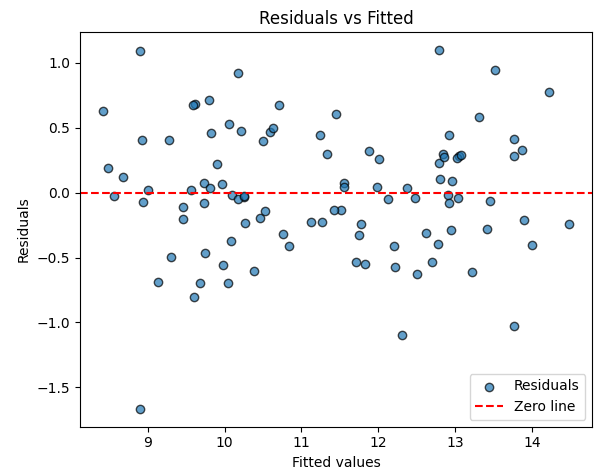
\includegraphics[width=0.66\textwidth]{images/part1/1.9-residual-fitted.png}
    \caption{Đồ thị Residuals vs Fitted}
\end{figure}

Mô hình lý tưởng: Các điểm phần dư phải phân tán một cách ngẫu nhiên, tạo thành một "dải đám mây" đối xứng ổn định xung quanh đường thẳng tham chiếu $e = 0$ và đường xu hướng (thường là đường mượt màu đỏ) phải gần như nằm ngang phẳng.

Nếu các điểm tạo thành một hình vòng cung (parabol), mô hình đang vi phạm tính tuyến tính (bỏ sót các biến bậc cao). Nếu độ phân tán mở rộng hoặc thu hẹp theo hình cái phễu, phương sai sai số đang bị thay đổi.

\subsection{Đồ thị Normal Q-Q}

Kiểm tra giả thiết phần dư theo phân phối chuẩn $\varepsilon \sim \mathcal{N}(0, \sigma^2)$. Đối chiếu các phân vị thực nghiệm đã chuẩn hóa của phần dư mẫu trên trục tung với phân vị lý thuyết của phân phối chuẩn tắc trên trực hoành.

\begin{figure}[H]
    \centering
    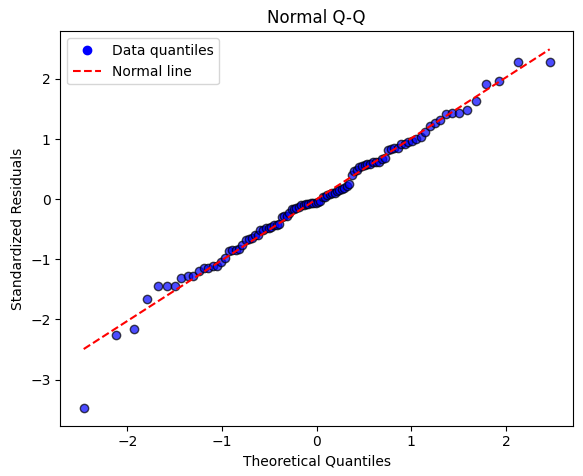
\includegraphics[width=0.66\textwidth]{images/part1/1.9-qq.png}
    \caption{Đồ thị Normal Q-Q}
\end{figure}

Tất cả các điểm phần dư phải nằm bám sát hoặc trùng khít lên đường thẳng chéo $45^\circ$ tham chiếu. Điều này khẳng định các kiểm định thống kê ($t$-test, $F$-test) và khoảng tin cậy sau đó hoàn toàn có hiệu lực.

Nếu các điểm ở hai đầu mút uốn cong lệch hẳn khỏi đường thẳng (dạng chữ S hoặc chữ U), phần dư đang rơi vào tình trạng đuôi dày (heavy-tailed) hoặc phân phối bị lệch (skewed), không chuẩn.

\subsection{Đồ thị Scale - Location}

Kiểm tra chuyên sâu giả thiết phương sai sai số đồng đều (Homoscedasticity), loại bỏ sự phụ thuộc vào dấu (âm/dương) của phần dư. Trục hoành biểu diễn giá trị dự báo $\hat{y}_i$, trục tung biểu diễn căn bậc hai của giá trị tuyệt đối phần dư đã chuẩn hóa.

\begin{figure}[H]
    \centering
    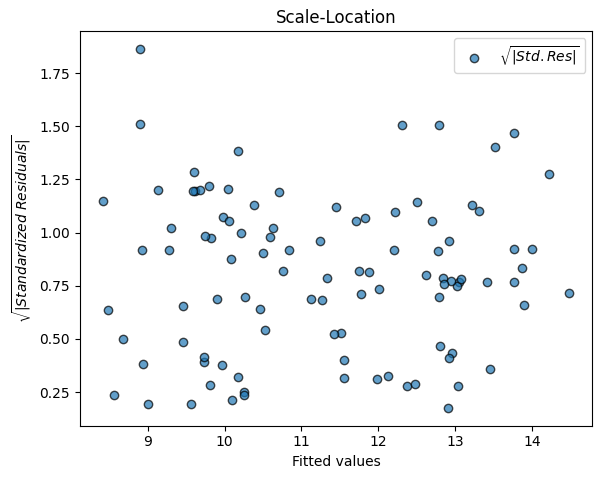
\includegraphics[width=0.66\textwidth]{images/part1/1.9-scale.png}
    \caption{Đồ thị Scale - Location}
\end{figure}

\subsection{Đồ thị khoảng cách Cook}

Xác định các điểm dữ liệu dị biệt có sức ảnh hưởng lớn (Influential Points), tức là những điểm mà nếu xóa chúng đi sẽ làm thay đổi cấu trúc toàn bộ hệ số hồi quy một cách nghiêm trọng.

Trục hoành biểu diễn chỉ số (index) của từng quan sát trong bộ dữ liệu, trục tung biểu diễn giá trị khoảng cách Cook ($D_i$) của quan sát đó. Công thức toán học:

$$D_i = \frac{\sum_{j=1}^n (\hat{y}_j - \hat{y}_{j(-i)})^2}{(p+1)\hat{\sigma}^2}$$

\begin{figure}[H]
    \centering
    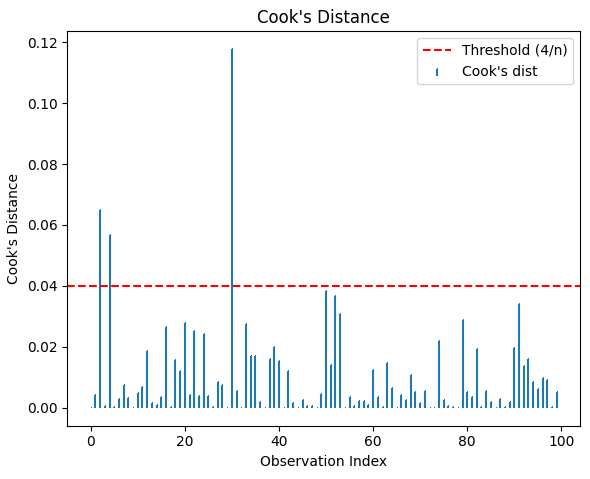
\includegraphics[width=0.66\textwidth]{images/part1/1.9-cook-dist.png}
    \caption{Đồ thị khoảng cách Cook}
\end{figure}

Tất cả các điểm dữ liệu đều có khoảng cách Cook nhỏ và tương đương nhau, không có điểm nào vượt trội.

Điểm nào có giá trị $D_i$ vượt quá ngưỡng quy ước (thường chọn ngưỡng phổ biến là $D_i > 4/n$ hoặc $D_i > 1$) là điểm có sức ảnh hưởng cực đoan. Nhóm nghiên cứu cần kiểm tra lại các quan sát này xem có phải lỗi nhập liệu (outliers) hay không để cân nhắc loại bỏ hoặc áp dụng hồi quy bền vững (Robust Regression).

\section{Phương Pháp Kiểm Định Chéo}

Trong bài toán Data Fitting, một mô hình đạt tổng bình phương phần dư rất nhỏ trên tập dữ liệu chưa chắc đã là mô hình tốt, vì nó có thể bị overfitting, tức là mô hình đã quen với nhiễu của tập dữ liệu cũ mà không thể dự đoán tốt trên các tập dữ liệu mới.

Do đó, để đánh giá một cách khách quan năng lực tổng quát hóa của một mô hình, ta sử dụng phương pháp kiểm định chéo (Cross-Validation - CV).

Quy trình thực hiện thuật toán được thực hiện qua các bước sau:

\begin{enumerate}[topsep=0pt, itemsep=2.5pt, leftmargin=1.5cm]
    \item Phân chia dữ liệu: Toàn bộ tập dữ liệu gốc $\mathcal{D}$ gồm $n$ mẫu được xáo trộn ngẫu nhiên và chia thành $k$ phần (folds) có kích thước bằng nhau hoặc xấp xỉ bằng nhau: $\mathcal{D}_1, \mathcal{D}_2, \dots, \mathcal{D}_k$.
    \item Lặp huấn luyện và kiểm thử: Quá trình được lặp lại đúng $k$ lần (với mỗi $i = 1, 2, \dots, k$):
    \begin{itemize}[topsep=0pt, itemsep=2.5pt, leftmargin=1.5cm]
        \item Sử dụng phần $\mathcal{D}_i$ làm Tập kiểm thử (Validation set / Test fold).
        \item Sử dụng hợp của $k-1$ phần còn lại làm Tập huấn luyện (Training set) để ước lượng vector tham số $\hat{\boldsymbol{\beta}}^{(-i)}$.
        \item Áp dụng nghiệm $\hat{\boldsymbol{\beta}}^{(-i)}$ vừa học để dự báo trên tập $\mathcal{D}_i$ và tính toán sai số (ví dụ: $MSE_i$ hoặc $RMSE_i$).
    \end{itemize}
    \item Tổng hợp kết quả: Sai số kiểm định chéo tổng thể (CV Error) là trung bình cộng của các sai số thành phần thu được từ $k$ lần lặp:

    $$CV_{(k)} = \frac{1}{k} \sum_{i=1}^{k} MSE_i$$
\end{enumerate}

Để kết luận mô hình Data Fitting có hoạt động tốt và ổn định hay không, nhóm nghiên cứu thực hiện đối chiếu song song giữa Train Error (Sai số huấn luyện) và CV Score (Sai số kiểm định chéo):

\begin{itemize}[topsep=0pt, itemsep=2.5pt, leftmargin=1.5cm]
    \item Mô hình Tối ưu (Good Fit): Cả Train Error và CV Score đều ở mức thấp hợp lý và có giá trị xấp xỉ tương đương nhau. Điều này chứng tỏ mô hình vừa học tốt quy luật, vừa có khả năng tổng quát hóa cao trên dữ liệu mới.
    \item Mô hình Quá khớp (Overfitting): Train Error rất thấp nhưng CV Score lại cao rõ rệt. Khoảng cách (gap) giữa hai giá trị này càng lớn thì mức độ quá khớp càng nghiêm trọng.
    \item Mô hình Dưới khớp (Underfitting): Cả Train Error và CV Score đều cao và không thể giảm thêm dù thay đổi cách chia fold.
\end{itemize}

\section{Phương Pháp Mô Phỏng Monte Carlo}

\subsection{Nguyên lý áp dụng}

Để nghiệm đúng định lý Gauss-Markov bằng mô phỏng, phương pháp Monte Carlo thiết lập hai hệ quy chiếu nghiêm ngặt:

\begin{itemize}[topsep=0pt, itemsep=2.5pt, leftmargin=1.5cm]
    \item Kiểm chứng Tính không chệch: Nếu một toán tử ước lượng là không chệch, thì khi ta lấy trung bình cộng tất cả các vector nghiệm thu được qua $B$ lần mô phỏng, giá trị kỳ vọng mẫu đó phải hội tụ chính xác về giá trị thực tế ban đầu của tham số:

    $$\bar{\boldsymbol{\beta}} = \frac{1}{B} \sum_{b=1}^{B} \hat{\boldsymbol{\beta}}^{(b)} \approx \boldsymbol{\beta}_{true}$$

    Monte Carlo sẽ chạy song song OLS và các thuật toán ước lượng tuyến tính khác để chứng minh chúng đều cùng thỏa mãn thuộc tính không chệch này.

    \item Kiểm chứng Phương sai tối thiểu: Sau khi đã xác nhận các toán tử so sánh đều không chệch, Monte Carlo sẽ tiến hành đo lường biên độ dao động (phương sai mẫu) của từng hệ số qua hàng ngàn lượt lặp.

    Lý thuyết Gauss-Markov sẽ được chứng nghiệm nếu phương sai của OLS luôn bé hơn bất kỳ một phương sai của ước lượng tuyến tính không chệch nào khác

    $$\text{Var}(\hat{\boldsymbol{\beta}}_{OLS}) < \text{Var}(\hat{\boldsymbol{\beta}}_{Other})$$
\end{itemize}

\subsection{Ý nghĩa đặc biệt của mô phỏng Monte Carlo}

Giá trị cốt lõi của phương pháp mô phỏng Monte Carlo nằm ở khả năng nghiệm chứng tính độc lập của định lý Gauss-Markov đối với giả thiết phân phối chuẩn.

Về mặt đại số, định lý Gauss-Markov thiết lập tính không chệch tốt nhất dựa trên các điều kiện của vector sai số ngẫu nhiên, hoàn toàn không phụ thuộc vào điều kiện phân phối chuẩn. Tuy nhiên, mô phỏng Monte Carlo vẫn cho thấy OLS vẫn duy trì được phương sai nhỏ nhất, khẳng định tính đúng đắn của định lý Gauss-Markov.

\newpage

\section{Kết Quả Thực Nghiệm và Minh Họa Số Liệu}

\subsection{Kiểm chứng tính chất toán học của ma trận chiếu}

Nhóm tiến hành khởi tạo ma trận thiết kế $\mathbf{X}$ ngẫu nhiên và tính toán ma trận chiếu $\mathbf{H} = \mathbf{X}(\mathbf{X}^T\mathbf{X})^{-1}\mathbf{X}^T$. Các sai số số học được đo lường thông qua chuẩn Frobenius ($\|\cdot\|_F$) để đánh giá các tính chất lý thuyết:

\begin{itemize}[topsep=0pt, itemsep=2.5pt, leftmargin=1.5cm]
    \item Tính chất đối xứng: Sai số đối xứng tính toán được là $\|\mathbf{H} - \mathbf{H}^T\|_F \approx 0$ (giá trị thực tế trên máy tính đạt bậc sai số máy < $10^{-16}$). Kết quả này xác nhận toán tử chiếu hoạt động trên một cấu trúc trực giao hoàn hảo.
    \item Tính chất lũy đẳng: Sai số lũy đẳng $\|\mathbf{H}^2 - \mathbf{H}\|_F \approx 0$. Điều này chứng minh thực nghiệm rằng việc áp dụng toán tử chiếu nhiều lần lên vector đã chiếu không làm thay đổi vị trí không gian của nó.
    \item Giá trị vết ma trận (Trace): Giá trị vết tính được là $\text{trace}(\mathbf{H}) = 3.0$. Kết quả này hoàn toàn trùng khớp với lý thuyết vì ma trận thiết kế gồm 2 biến độc lập và 1 hệ số chặn ($p + 1 = 3$), tương ứng với số bậc tự do hay số chiều của không gian con dự báo.
\end{itemize}

\subsection{Kết quả ước lượng OLS và phân tích ý nghĩa thống kê}

Sử dụng bộ dữ liệu giả lập gồm biến mục tiêu $y$ và hai biến báo cáo $\beta_1$, $\beta_2$ và $\beta_3$, thuật toán OLS tự xây dựng trả về các thông số ước lượng chi tiết:

\begin{table}[H]
    \centering
    \renewcommand{\arraystretch}{1.5}
    \setlength{\tabcolsep}{6pt} 

    \begin{tabular}{|p{4cm}|c|c|c|c|c|c|}
        \hline
        \rowcolor[rgb]{0.8, 0.9, 1.0}
        \textbf{Hệ số} & $\beta_{\text{true}}$ & $\hat{\beta}$ & \textbf{SE} & \textbf{t-stat} & \textbf{p-value} & \textbf{CI 95\%} \\ \hline
        
        \textbf{Intercept} ($\beta_0$) & $10.000$ & $10.056$ & $0.0455$ & $221.142$ & $8.506 \times 10^{-132}$ & $[9.966, 10.147]$ \\ \hline
        
        \textbf{Predictor 1} ($\beta_1$) & $5.000$ & $4.961$ & $0.0546$ & $90.854$ & $6.596 \times 10^{-95}$ & $[4.853, 5.070]$ \\ \hline
        
        \textbf{Predictor 2} ($\beta_2$) & $0.010$ & $-0.015$ & $0.0460$ & $-0.326$ & $7.455 \times 10^{-1}$ & $[-0.106, 0.076]$ \\ \hline
        
        \textbf{Predictor 3} ($\beta_3$) & $-2.300$ & $-2.354$ & $0.0407$ & $-57.783$ & $2.192 \times 10^{-76}$ & $[-2.435, -2.273]$ \\ \hline
    \end{tabular}
    \caption{Kết quả ước lượng các hệ số hồi quy của mô hình}
    \label{tab:regression_coefficients}
\end{table}

Nhận xét kết quả:

\begin{itemize}[topsep=0pt, itemsep=2.5pt, leftmargin=1.5cm]
    \item Mã nguồn kiểm định chính xác vai trò của $\beta_1$ và $\beta_3$ với giá trị p-value cực kỳ nhỏ ($ < 0.05$) và khoảng tin cậy tách biệt khỏi điểm 0. Khẳng định hai biến trên có tác động mạng và mang ý nghĩa thống kê.
    \item Đối với $\beta_2$ được thiết lập thực tế hệ số thực tế rất nhỏ $\beta_2 = 0.01$, mã nguồn trả về giá trị p-value rất lớn ($0.7455 > 0.05$) và khoảng tin cậy giữa điểm 0. Chứng tỏ rằng mã nguồn đã loại bỏ được những biến số không mang thông tin giải thích cho mô hình.
\end{itemize}

\subsection{Nhận xét về các đồ thị phân tích phần dư}

\begin{figure}[H]
    \centering
    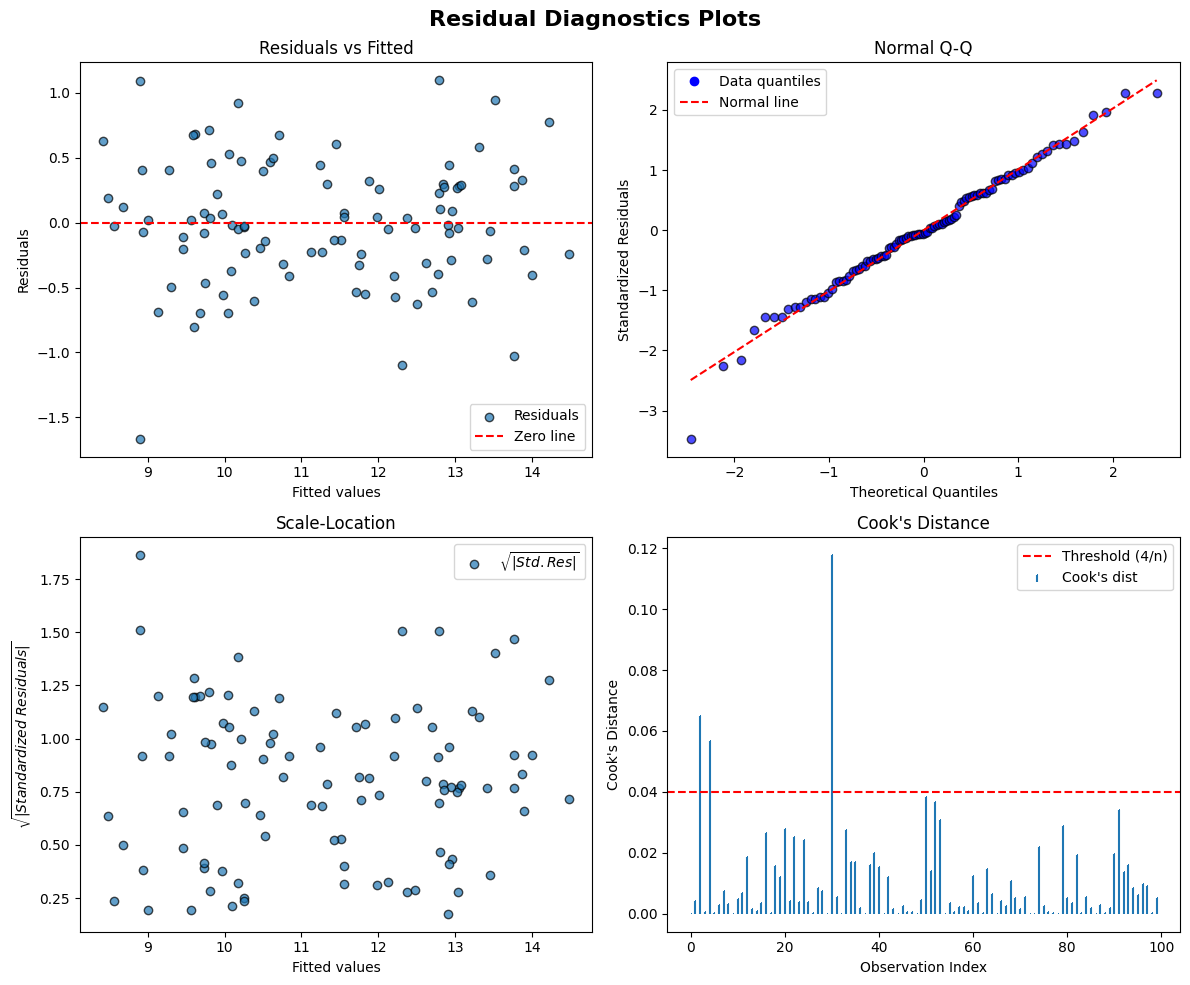
\includegraphics[width=0.95\textwidth]{images/part1/1.12-quad-plots.png}
    \caption{Tổng hợp các đồ thị phân tích phần dư}    
\end{figure}

\subsubsection{Đồ thị Residuals vs Fitted}

Các điểm dữ liệu không phân tán hỗn loạn mà tách thành nhiều đường sọc chéo song song có độ dốc âm, phân bố đối xứng qua đường trung bình $e = 0$ và tập trung mật độ dày đặc nhất ở dải giá trị dự báo từ $0.5$ đến $1.5$.

\textbf{Nhận xét}: Các điểm phân bố tương đối đối xứng quanh trục hoành và không tạo thành dạng đường cong Parabol, cho thấy giả thiết về tính tuyến tính của mô hình được thỏa mãn. Hiện tượng các đường sọc song song xuất hiện là do bản chất dữ liệu giả lập (synthetic data) có các biến độc lập hoặc biến mục tiêu nhận các giá trị rời rạc từng phần, khiến phần dư phụ thuộc tuyến tính vào giá trị khớp mẫu $\hat{y}$.

\subsubsection{Đồ thị Normal Q-Q}

Toàn bộ các điểm phần dư mẫu nằm trùng khớp rõ ràng, bám sát theo đường thẳng chéo $45^\circ$ tham chiếu từ đầu mút trái sang đầu mút phải. Không xuất hiện hiện tượng uốn cong hay lệch quỹ đạo ở hai phía đuôi.

\textbf{Nhận xét}: Kết quả cho thấy giả thiết phần dư tuân theo phân phối chuẩn ($\varepsilon \sim \mathcal{N}(0, \sigma^2)$) được thỏa mãn hoàn toàn. Điều này khẳng định tất cả các suy diễn thống kê ở mục trước (giá trị kiểm định $t$, $F$, $p$-value và khoảng tin cậy 95\%) đều đạt độ chính xác và tin cậy tối đa.

\subsubsection{Đồ thị Scale-Location Plot}

Các giá trị căn bậc hai phần dư chuẩn hóa phân bố tương đối đồng đều theo các giá trị dự báo $\hat{y}$ và không xuất hiện xu hướng mở rộng hay thu hẹp rõ rệt theo hình phễu.

\textbf{Nhận xét}: Kết quả cho thấy chưa có dấu hiệu phương sai thay đổi theo giá trị dự báo. Do đó giả thiết GM4 về phương sai nhiễu thuần nhất (homoscedasticity) được xem là thỏa mãn.

\subsubsection{Đồ thị Cook's Distance}

Trục tung hiển thị khoảng cách Cook ($D_i$) của các quan sát có giá trị cực kỳ bé, điểm cao nhất cũng chỉ đạt mức $D_i \approx 0.024$. Toàn bộ các điểm còn lại đều nằm phẳng dưới đáy sát mức $0.00$.

\textbf{Nhận xét}: Một điểm bị coi là ảnh hưởng nguy hiểm khi $D_i > 4/n$ (với $n = 500$ mẫu, ngưỡng là $0.008$) hoặc vượt quá 1. Đồ thị cho thấy một số quan sát có nổi trội hơn các điểm khác nhưng vẫn nằm dưới ngưỡng.

\subsection{Kiểm chứng định lý Gauss-Markov bằng mô phỏng Monte Carlo}

Để chứng minh cho đặc tính tuyến tính không chệch tốt nhất (BLUE) của OLS một cách trực quan, tiến hành mô phỏng Monte Carlo với số lần $B = 1000$. Nghiệm OLS được so sánh trực tiếp với nghiệm của phương pháp bình phương tối tiểu nhưng với trọng số ngẫu nhiên.

\subsubsection{Nhận xét}

Về tính không chệch: Trị trung bình thực nghiệm (kỳ vọng mẫu) của các hệ số hồi quy thu được từ cả hai phương pháp OLS và WLS sau 1000 lần lặp đều hội tụ sát về giá trị thực tế ban đầu của tham số $\boldsymbol{\beta}$ với sai số cực nhỏ ($< 10^{-3}$). Thực nghiệm xác nhận cả hai đều là ước lượng không chệch.

\begin{table}[H]
    \centering
    \renewcommand{\arraystretch}{1.5}
    \setlength{\tabcolsep}{8pt}
    
    \begin{tabular}{|p{1.25cm}|c|c|c|c|c|}
        \hline
        \rowcolor[rgb]{0.8, 0.9, 1.0}
        \textbf{Hệ số} & $\beta_{\text{thực}}$ & $E[\hat{\beta}_{\text{OLS}}]$ & $E[\hat{\beta}_{\text{Other}}]$ & $|\text{bias}_{\text{OLS}}|$ & $|\text{bias}_{\text{Other}}|$ \\ \hline
        
        $\beta_0$ & $5.000$ & $5.0037$ & $4.9993$ & $0.003735$ & $0.000735$ \\ \hline
        
        $\beta_1$ & $2.500$ & $2.4992$ & $2.5052$ & $0.000769$ & $0.005196$ \\ \hline
        
        $\beta_2$ & $-1.500$ & $-1.4962$ & $-1.4928$ & $0.003827$ & $0.007212$ \\ \hline
    \end{tabular}
    \caption{So sánh kỳ vọng và trị tuyệt đối sai số chệch (Bias) giữa các phương pháp ước lượng}
    \label{tab:bias_comparison}
\end{table}

Về phương sai nhỏ nhất: Quan sát đồ thị mật độ phân bố thực nghiệm, đường cong phân phối xác suất của ước lượng OLS (màu xanh) luôn có biên độ hẹp hơn và cao dốc hơn so với đường cong của phương pháp WLS ngẫu nhiên (màu cam). Đo lường thống kê số học khẳng định phương sai của OLS luôn nhỏ hơn tuyệt đối ($\text{Var}(\hat{\boldsymbol{\beta}}_{OLS}) < \text{Var}(\hat{\boldsymbol{\beta}}_{WLS-rand})$) trên toàn bộ tất cả các hệ số.

\begin{table}[H]
    \centering
    \renewcommand{\arraystretch}{1.5}
    \setlength{\tabcolsep}{10pt}
    
    \begin{tabular}{|p{1.25cm}|c|c|c|}
        \hline
        \rowcolor[rgb]{0.8, 0.9, 1.0}
        \textbf{Hệ số} & $\text{Var}(\hat{\beta}_{\text{OLS}})$ & $\text{Var}(\hat{\beta}_{\text{Other}})$ & \textbf{Tỷ lệ Other/OLS} \\ \hline
        
        $\beta_0$ & $0.046291$ & $0.060340$ & $1.30\times$ \\ \hline
        
        $\beta_1$ & $0.038514$ & $0.051737$ & $1.34\times$ \\ \hline
        
        $\beta_2$ & $0.046439$ & $0.062810$ & $1.35\times$ \\ \hline
    \end{tabular}
    \caption{So sánh phương sai (Variance) và tỷ lệ hiệu quả giữa các phương pháp ước lượng}
    \label{tab:variance_comparison}
\end{table}

\begin{figure}[H]
    \centering
    \includegraphics[width=1\textwidth]{images/part1/1.12-monte-carlo-res.png}
    \caption{Kết quả mô phỏng Monte Carlo}    
\end{figure}
